%%%%%%%%%%%%%%%%%%%%%%%%%%%%%%%%%%%%%%%%%
% Short Sectioned Assignment
% LaTeX Template
% Version 1.0 (5/5/12)
%
% This template has been downloaded from:
% http://www.LaTeXTemplates.com
%
% Original author:
% Frits Wenneker (http://www.howtotex.com)
%
% License:
% CC BY-NC-SA 3.0 (http://creativecommons.org/licenses/by-nc-sa/3.0/)
%
%%%%%%%%%%%%%%%%%%%%%%%%%%%%%%%%%%%%%%%%%

%----------------------------------------------------------------------------------------
%	PACKAGES AND OTHER DOCUMENT CONFIGURATIONS
%----------------------------------------------------------------------------------------

\documentclass[paper=a4, fontsize=11pt]{scrartcl} % A4 paper and 11pt font size

\usepackage[T1]{fontenc} % Use 8-bit encoding that has 256 glyphs
\usepackage{fourier} % Use the Adobe Utopia font for the document - comment this line to return to the LaTeX default
\usepackage[english]{babel} % English language/hyphenation
\usepackage{amsmath,amsfonts,amsthm} % Math packages
\usepackage{subcaption}

\usepackage{graphicx}

\usepackage{lipsum} % Used for inserting dummy 'Lorem ipsum' text into the template

\usepackage{sectsty} % Allows customizing section commands
\allsectionsfont{\centering \normalfont\scshape} % Make all sections centered, the default font and small caps

\usepackage{fancyhdr} % Custom headers and footers
\pagestyle{fancyplain} % Makes all pages in the document conform to the custom headers and footers
\fancyhead{} % No page header - if you want one, create it in the same way as the footers below
\fancyfoot[L]{} % Empty left footer
\fancyfoot[C]{} % Empty center footer
\fancyfoot[R]{\thepage} % Page numbering for right footer
\renewcommand{\headrulewidth}{0pt} % Remove header underlines
\renewcommand{\footrulewidth}{0pt} % Remove footer underlines
\setlength{\headheight}{13.6pt} % Customize the height of the header

\numberwithin{equation}{section} % Number equations within sections (i.e. 1.1, 1.2, 2.1, 2.2 instead of 1, 2, 3, 4)
\numberwithin{figure}{section} % Number figures within sections (i.e. 1.1, 1.2, 2.1, 2.2 instead of 1, 2, 3, 4)
\numberwithin{table}{section} % Number tables within sections (i.e. 1.1, 1.2, 2.1, 2.2 instead of 1, 2, 3, 4)

\setlength\parindent{0pt} % Removes all indentation from paragraphs - comment this line for an assignment with lots of text

%----------------------------------------------------------------------------------------
%	TITLE SECTION
%----------------------------------------------------------------------------------------

\newcommand{\horrule}[1]{\rule{\linewidth}{#1}} % Create horizontal rule command with 1 argument of height

\title{	
\normalfont \normalsize 
\textsc{McGill University, Department of Electrical and Computer Engineering} \\ [25pt] % Your university, school and/or department name(s)
\horrule{0.5pt} \\[0.4cm] % Thin top horizontal rule
\huge Assignment 2: Where are the Airplanes? \\ % The assignment title
\horrule{2pt} \\[0.5cm] % Thick bottom horizontal rule
}

\author{Prof. Alexandre Zaghetto} % Your name

\date{\normalsize\today} % Today's date or a custom date

\begin{document}

\maketitle % Print the title

%----------------------------------------------------------------------------------------
%	PROBLEM 1
%----------------------------------------------------------------------------------------

\section{Image Denoising}
\label{denoise}

In this assignment you will implement an image processing algorithm to determine the approximate location of parked air planes in a zoomed part of the Dallas/Fort Worth International Airport. The satellite $RGB$ images you have access to have their $Y$ (luminance), $C_b$ and $C_r$ (chrominances) components corrupted by Gaussian noise, impulsive salt-and-paper noise and texture caused by the presence of an unwanted frequency components, respectively. The first step of your algorithm is to generate a single denoised image. Figure\ref{fig:airport} (a) and (b) show examples of a noisy and a denoised image, respectively. To perform this task, use spatial and frequency domain filtering. With the exception of the Fast Fourier Transform, do not use any built-in function to perform filtering.


\begin{figure}[h]
	\centering
	\begin{subfigure}[b]{0.35\textwidth}
		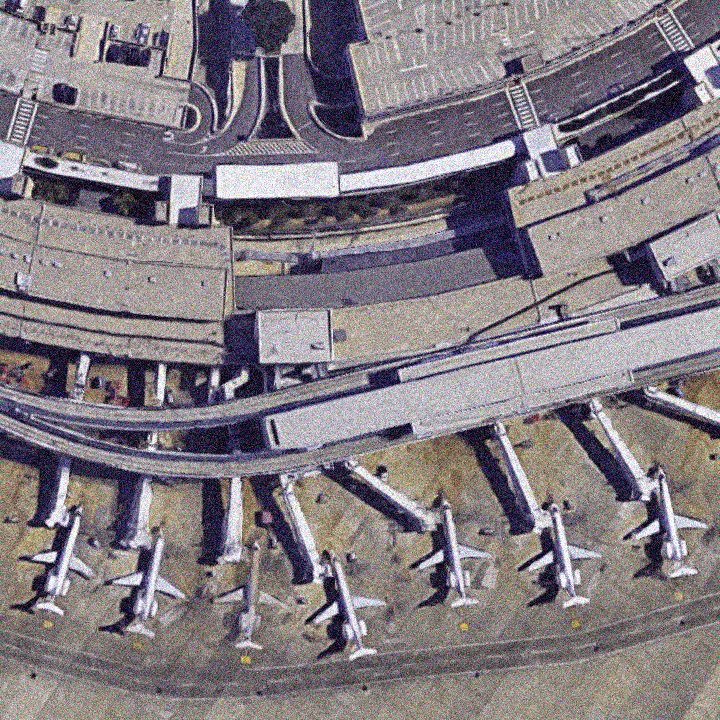
\includegraphics[width=5cm]{noisy.png}
		\label{fig:noisy}
	\end{subfigure}
	 \hspace{2eM}
	 \centering
	\begin{subfigure}[b]{0.35\textwidth}
	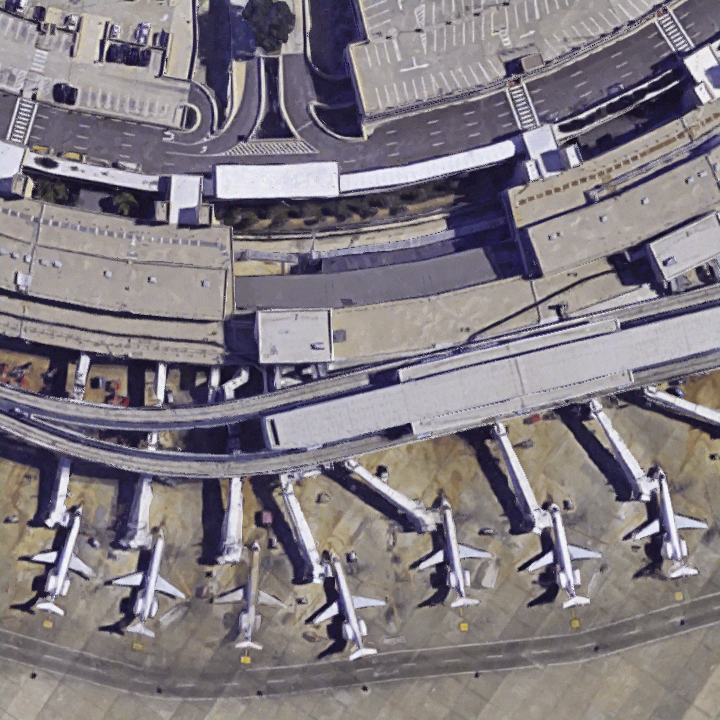
\includegraphics[width=5cm]{denoised.png}
	\label{fig:denoised}
	\end{subfigure}
	\caption{Zoomed part of the Dallas/Fort Worth International Airport: (a) noisy image; and (b) denoised image.}
	\label{fig:airport}
\end{figure}


\clearpage
%------------------------------------------------
\section{Finding the Airplanes}
%------------------------------------------------

Next you will use the denoised image generate in Section~\ref{denoise} to find where the airplanes are parked. First you must manually define an airplane template. Figure~\ref{fig:template} shows an example. Airplanes must be found via correlation in the $YC_bC_r$ color space (you must implement the convolution algorithm). You will need to generate slightly rotated versions of your template in order to contemplate all the airplanes that appear in the image (you may use any built-in function to perform image rotation). Taking a vertical axis as the reference, rotate the template from $-45^\circ$ to $45^\circ$ using $9^\circ$ increments. The output of your algorithm are the approximate locations of the airplanes. You are free to propose additional techniques to improve the accuracy of your algorithm.  

\begin{figure}[h]
	\centering
	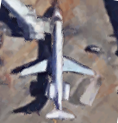
\includegraphics[width=0.2\textwidth]{airplane.png}
	\caption{Airplane template.}
	\label{fig:template}
\end{figure}

%\begin{figure}
%	\centering
%	\begin{subfigure}[b]{0.4\textwidth}
%		\fbox{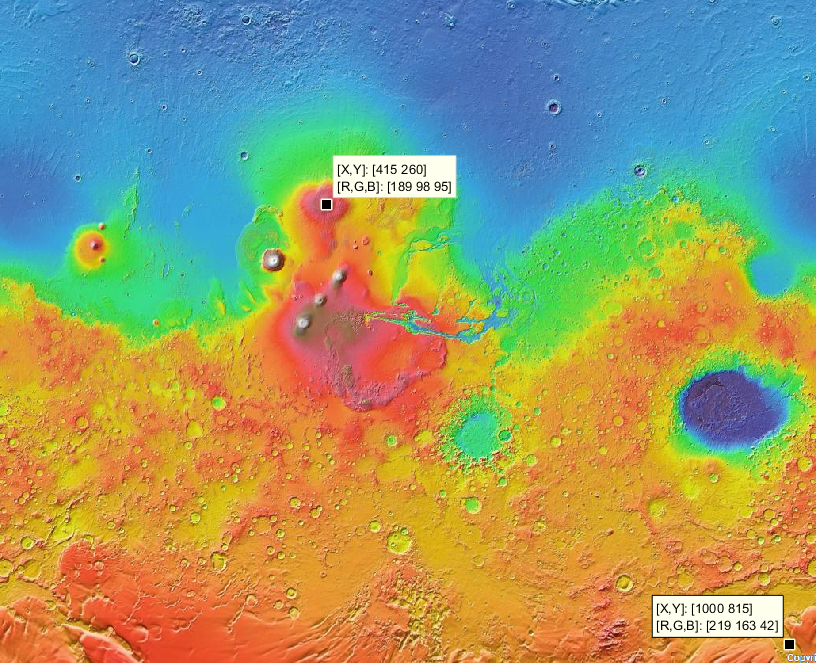
\includegraphics[height=5cm]{mars.png}}
%		\caption{}
%		\label{fig:mars}
%	\end{subfigure}
%	~ %add desired spacing between images, e. g. ~, \quad, \qquad, \hfill etc. 
%	%(or a blank line to force the subfigure onto a new line)
%	\hspace{3eM}
%	\begin{subfigure}[b]{0.4\textwidth}
%		\fbox{
\includegraphics[height=5cm]{spots.png}}
%		\caption{}
%		\label{fig:spots}
%	\end{subfigure}
%	\caption{(a) Base location and supplies landing zone; and (b) potential microorganisms.}\label{fig:animals}
%	\label{fig:two}
%\end{figure}





\end{document}